\documentclass{beamer}

\input{settings.tex}


\title{Sums of Squares Programming}
\subtitle{Advanced Control}
\author{by Sergei Savin}
\centering
\date{\mydate}



\begin{document}
\maketitle


\begin{frame}{Content}
\begin{itemize}
	\item Convex Functions
	\item Convex Regions
	\item Convex Optimization
	\item Properties of Convex Optimization
	\item Sum of Squares
	\item Polynomial Basis
	\item Gram Matrix
	\item Sum of Squares Programming
	\item Monomial Basis SoS Programming
\end{itemize}
\end{frame}

\begin{frame}
	\begin{center}
		{\Large Part 1: Convex Optimization}
	\end{center}
\end{frame}

\begin{frame}{Convex Functions}
	\begin{flushleft}
		A convex function is ``shaped like a bowl'':
		
		\bigskip
		
		Any straight line drawn between two points on its curve stays entirely
		\textbf{above} (or along) the curve itself.
		
		\bigskip
		
		Equivalently, any tangent to the function stays
		\textbf{below} (or along) its curve.
		
		\vspace{-2.5em}
		
		\begin{center}
			\begin{minipage}[t]{.4\textwidth}
				\centering
				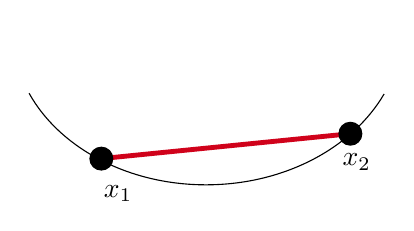
\begin{tikzpicture}[x=0.75pt,y=0.75pt,yscale=-1,xscale=1]
					\draw [draw opacity=0, line width=1.0pt] (696.23,142.36) .. controls (681.43,167.71) and (649.5,185.54) .. (612.24,186.11) .. controls (573.51,186.7) and (539.97,168.5) .. (525.19,141.99) -- (611.08,111.08) -- cycle ;
					\draw (696.23,142.36) .. controls (681.43,167.71) and (649.5,185.54) .. (612.24,186.11) .. controls (573.51,186.7) and (539.97,168.5) .. (525.19,141.99) ;
					\draw [color={rgb, 255:red, 208; green, 2; blue, 27}, draw opacity=1, line width=1.75pt] (680,161.5) -- (560,173.5) ;
					\draw [color={rgb, 255:red, 208; green, 2; blue, 27}, draw opacity=1] (680,161.5) -- (560,173.5) ;
					%Shape: Circle [id:dp3160827101885906]
					\draw [fill={rgb, 255:red, 0; green, 0; blue, 0}, fill opacity=1] (554.5,173.5) .. controls (554.5,170.46) and (556.96,168) .. (560,168) .. controls (563.04,168) and (565.5,170.46) .. (565.5,173.5) .. controls (565.5,176.54) and (563.04,179) .. (560,179) .. controls (556.96,179) and (554.5,176.54) .. (554.5,173.5) -- cycle ;
					%Shape: Circle [id:dp16415395117171228]
					\draw [fill={rgb, 255:red, 0; green, 0; blue, 0}, fill opacity=1] (674.5,161.5) .. controls (674.5,158.46) and (676.96,156) .. (680,156) .. controls (683.04,156) and (685.5,158.46) .. (685.5,161.5) .. controls (685.5,164.54) and (683.04,167) .. (680,167) .. controls (676.96,167) and (674.5,164.54) .. (674.5,161.5) -- cycle ;
					\draw (560,185) node [anchor=north west, inner sep=0.75pt, align=left] {$x_1$};
					\draw (675,170) node [anchor=north west, inner sep=0.75pt, align=left] {$x_2$};
				\end{tikzpicture}
				\captionof{figure}{Convex function}
			\end{minipage}%
			\begin{minipage}[t]{.7\textwidth}
				\centering
				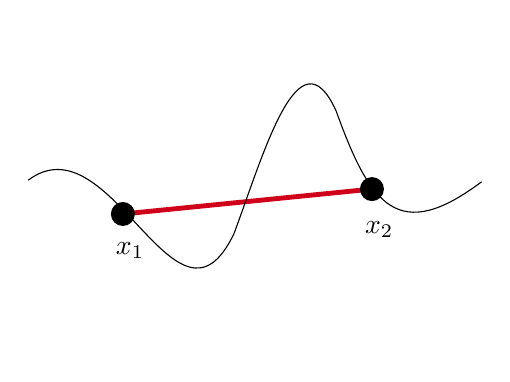
\begin{tikzpicture}[x=0.75pt,y=0.75pt,yscale=-1,xscale=1]
					%Straight Lines [id:da6875192047258083]
					\draw [color={rgb, 255:red, 208; green, 2; blue, 27}, draw opacity=1, line width=1.75pt] (564.6,165.5) -- (444.6,177.5) ;
					%Shape: Circle [id:dp14324656781298462]
					\draw [fill={rgb, 255:red, 0; green, 0; blue, 0}, fill opacity=1] (439.1,177.5) .. controls (439.1,174.46) and (441.56,172) .. (444.6,172) .. controls (447.64,172) and (450.1,174.46) .. (450.1,177.5) .. controls (450.1,180.54) and (447.64,183) .. (444.6,183) .. controls (441.56,183) and (439.1,180.54) .. (439.1,177.5) -- cycle ;
					%Shape: Circle [id:dp2582069443071713]
					\draw [fill={rgb, 255:red, 0; green, 0; blue, 0}, fill opacity=1] (559.1,165.5) .. controls (559.1,162.46) and (561.56,160) .. (564.6,160) .. controls (567.64,160) and (570.1,162.46) .. (570.1,165.5) .. controls (570.1,168.54) and (567.64,171) .. (564.6,171) .. controls (561.56,171) and (559.1,168.54) .. (559.1,165.5) -- cycle ;
					%Curve Lines [id:da47039197462224447]
					\draw (498.2,186.8) .. controls (512.6,148) and (529.4,88) .. (547.4,128) ;
					%Curve Lines [id:da13389450894014865]
					\draw (399,161.2) .. controls (439,131.2) and (470.6,244.8) .. (498.2,186.8) ;
					%Curve Lines [id:da2313253314744761]
					\draw (547.4,128) .. controls (563.8,173.6) and (577.4,192) .. (617.4,162) ;
					\draw (440,190) node [anchor=north west, inner sep=0.75pt, align=left] {$x_1$};
					\draw (560,180) node [anchor=north west, inner sep=0.75pt, align=left] {$x_2$};
				\end{tikzpicture}
				\captionof{figure}{Non-convex function}
			\end{minipage}
		\end{center}
		
	\end{flushleft}
\end{frame}

\begin{frame}{Convex Regions}
	\begin{flushleft}

					A \emph{convex} region is a shape or space where a straight line segment
			connecting any two points inside the region stays entirely inside it.
		
		\bigskip
		
		\begin{figure}
			\centering
			\begin{minipage}{.3\textwidth}
				\centering
				
				\textit{  
					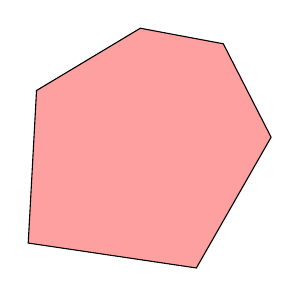
\begin{tikzpicture}[x=0.75pt,y=0.75pt,yscale=-1,xscale=1]
						\draw  [fill={rgb, 255:red, 255; green, 160; blue, 160 }  ,fill opacity=1 ] (148,55) -- (188,62.5) -- (211,107.5) -- (175,170.5) -- (94,158.5) -- (98,85) -- cycle ;
				\end{tikzpicture}}
				
				\captionof{figure}{Convex region}
			\end{minipage}%
			\begin{minipage}{.7\textwidth}
				\centering
				
				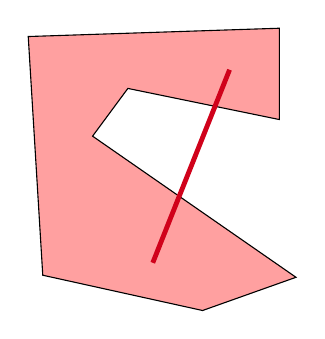
\begin{tikzpicture}[x=0.75pt,y=0.75pt,yscale=-1,xscale=1]
					\draw  [fill={rgb, 255:red, 255; green, 160; blue, 160 }  ,fill opacity=1 ] (525,68.5) -- (525,112.5) -- (452,97.5) -- (435,120.5) -- (533,188.5) -- (488,204.5) -- (411,187.5) -- (404,72.5) -- cycle ;
					\draw [color={rgb, 255:red, 208; green, 2; blue, 27 }  ,draw opacity=1, line width=1.75pt ]   (501,88.5) -- (486.03,126.12) -- (464,181.5) ;
				\end{tikzpicture}
				
				\captionof{figure}{Non-convex region}
			\end{minipage}
		\end{figure}
		
	\end{flushleft}
\end{frame}


\begin{frame}{Convex Optimization}
	\begin{flushleft}
		A problem of the form
		\[
		\begin{aligned}
			\underset{x}{\text{minimize}}\quad & f(x)\\
			\text{subject to}\quad & g_i(x) \leq 0,\\
			& h_j(x) = 0
		\end{aligned}
		\]
		is called \textbf{convex} if
		
		\begin{itemize}
			\item $f(x)$ is a convex function,
			\item each $g_i(x)$ is a convex function,
			\item each $h_j(x)$ is an affine function.
		\end{itemize}
		
		\bigskip
		
		For example:
		\[
		\begin{aligned}
			\underset{x}{\text{minimize}}\quad &(x+1)^2\\
			\text{subject to}\quad &x \geq 0.
		\end{aligned}
		\]
		
	\end{flushleft}
\end{frame}


\begin{frame}{Properties of Convex Optimization}
	\begin{flushleft}
		\begin{itemize}
			\item A \textbf{local minimum is a global minimum}.
			
			\bigskip
			
			\item Convex problems can often be solved \textbf{efficiently}, even for
			large numbers of variables.
			
			\bigskip
			
			\item There are \textbf{reliable algorithms} with strong theoretical
			guarantees.
			
			\bigskip
			
			\item There are mature \textbf{solvers}: software packages designed
			to solve specific classes of convex optimization problems.
		\end{itemize}
		
	\end{flushleft}
\end{frame}


\begin{frame}
	\begin{center}
		{\Large Part 2: Sum of Squares}
	\end{center}
\end{frame}


\begin{frame}{Sum of Squares}
	\begin{flushleft}
		Some polynomials can be represented as a \emph{sum of squares} (SoS):
		\[
		p(x) = \sum_i g_i(x)^2,
		\]
		where $g_i(x)$ are themselves polynomials.
		
		\bigskip
		
		An SoS polynomial is always \textbf{non-negative}:
		\[
		p(x) \geq 0 \qquad \text{for all }x.
		\]
		
		\bigskip
		
		\begin{itemize}
			\item For a general polynomial, checking whether it is non-negative
			can be computationally difficult (NP-hard in general).
		
			
			\item Checking whether a polynomial is SoS can be cast as a
			\textbf{convex optimization problem}.
			
			\item This gives us a practical way of finding
			\textbf{certificates of non-negativity}.
		\end{itemize}
		
	\end{flushleft}
\end{frame}


\begin{frame}{Polynomial Basis}
	\begin{flushleft}
		
		Let us define a collection of polynomials
		\[
		g_1(x),\;g_2(x),\;\ldots,\;g_N(x)
		\]
		and collect them into a vector
		\[
		g(x)=
		\begin{bmatrix}
			g_1(x)\\
			\vdots\\
			g_N(x)
		\end{bmatrix}.
		\]
		
		\bigskip
		
		We can use this vector to construct polynomials from products
		$g_i(x)g_j(x)$ with weights $q_{ij}$:
		\[
		p(x)=\sum_{i=1}^N\sum_{j=1}^N
		q_{ij}g_i(x)g_j(x).
		\]
		
		\bigskip
		
		Same, in matrix form:
		\[
		p(x)=g(x)^\top Qg(x).
		\]
		
		
	\end{flushleft}
\end{frame}




\begin{frame}{Polynomial Basis: example}
	\begin{flushleft}
		
		
		Consider a polynomial basis $g(x)$ and a Gram matrix $Q$:
		
		\[
		g(x)=
		\begin{bmatrix}
			1\\x
		\end{bmatrix},
		\qquad
		Q=
		\begin{bmatrix}
			2&1\\
			1&2
		\end{bmatrix}.
		\]
		
		Then we can constract a polynomial:
		\[
		\begin{aligned}
			p(x)
			&=
			\begin{bmatrix}1&x\end{bmatrix}
			\begin{bmatrix}2&1\\1&2\end{bmatrix}
			\begin{bmatrix}1\\x\end{bmatrix}\\
			&=2+2x+2x^2.
		\end{aligned}
		\]
		
	\end{flushleft}
\end{frame}



\begin{frame}{Gram Matrix}
	\begin{flushleft}
		In the expression $p(x)=g(x)^\top Qg(x)$, the matrix $Q$ is called a \textbf{Gram matrix}.
		
		\begin{theorem}
			If $Q$ is symmetric and positive semidefinite, $Q \succeq 0$, then $p(x)=g(x)^\top Qg(x) \geq 0$ for all $x$.
		\end{theorem}
		
		\textbf{Proof:} For any choice of $x$, let $v=g(x)$. Since $Q\succeq0$, then $v^\top Qv\geq0$. Therefore, $p(x)=g(x)^\top Qg(x)\geq0.$ \qed
		
		\bigskip
		
		If $Q\succ0$ and $g(x)\neq0$ for all $x$, then $p(x)>0$ for all $x$.
		
	\end{flushleft}
\end{frame}


\begin{frame}{Gram Matrix: Example}
	\begin{flushleft}
		
		For
		\[
		g(x)=
		\begin{bmatrix}
			1\\x
		\end{bmatrix},
		\qquad
		Q=
		\begin{bmatrix}
			2&1\\
			1&2
		\end{bmatrix},
		\]
		the eigenvalues of $Q$ are
		\[
		\lambda_1=2+1=3>0,
		\qquad
		\lambda_2=2-1=1>0.\footnotemark
		\]
		%
		All eigenvalues are positive, so $Q\succ0$ (the matrix is positive definite).

		
		\bigskip
		
		Since $g(x)\neq0$ for any $x$, then $p(x)=g(x)^\top Qg(x)>0$ for all $x$. Indeed:
		\[
		p(x)=2+2x+2x^2>0.
		\]
		
		
		\footnotetext{\vspace{1.0em}
			For matrices of the form
			$\begin{bmatrix}a&b\\b&a\end{bmatrix}$,
			the eigenvalues are $a+b$ and $a-b$.}
			
	\end{flushleft}
\end{frame}


\begin{frame}{Example: Checking Positive-Definiteness}
	\begin{flushleft}
		Consider $p(x)=3x_1^2+4x_1x_2+3x_2^2+5$. Using the monomial basis:
		\[
		v(x)=
		\begin{bmatrix}
			x_1\\x_2\\1
		\end{bmatrix},
		\]
		the polynomial can be written as:
		\[
		p(x)=v(x)^\top Qv(x), \quad 
		Q=
		\begin{bmatrix}
			3&2&0\\
			2&3&0\\
			0&0&5
		\end{bmatrix}.
		\]
		
		The upper-left block has eigenvalues
		\[
		3+2=5>0,
		\qquad
		3-2=1>0.
		\]
		
		The eigenvalues of a block-diagonal matrix are the eigenvalues
		of its blocks, $\lambda(Q)=\{5,1,5\}$, so $Q \succ 0$. Thus:
		\[
		p(x)=v(x)^\top Qv(x)>0, \quad \forall x.
		\]
		
	\end{flushleft}
\end{frame}



\begin{frame}{Sum of Squares Programming}
	\begin{flushleft}
		Sum of squares (SoS) programming is a class of convex optimization
		problems that can include constraints of the type
		\[
		p(x) \in \mathrm{SoS}.
		\]
		
		\bigskip
		
		This means that we are looking for a matrix $Q$ such that
		\[
		Q\succeq0
		\]
		and
		\[
		p(x)=z(x)^\top Qz(x),
		\]
		where $z(x)$ is a fixed polynomial basis.
		
		\bigskip
		
		We can also require
		\[
		Q\succ0
		\]
		when we want a strictly positive polynomial.
		
	\end{flushleft}
	
\footnotetext{\vspace{1.0em}
		$Q \succ 0$ is often implemented as
		$Q\succeq\epsilon I$ for a small $\epsilon>0$.}
\end{frame}


\begin{frame}{Monomial Basis SoS Programming}
	\begin{flushleft}
		A common choice is to construct $z(x)$ from monomials up to
		some degree $N$:
		\[
		z(x)=
		\begin{bmatrix}
			1 & x_1 & x_2 & x_1x_2 & x_1^2 & x_2^2 & \cdots
		\end{bmatrix}^{\top}.
		\]
		
		\bigskip
		
		If $z(x)$ contains monomials up to degree $N$, then
		\[
		z(x)^\top Qz(x)
		\]
		can contain monomials up to degree $2N$.
		
		\bigskip
		
		For example, a polynomial of degree $2N$ can be written as
		\[
		p(x)=c_0+c_1x_1+c_2x_2+c_3x_1x_2
		+c_4x_1^2+\cdots.
		\]
		
		\bigskip
		
		We expand $z(x)^\top Qz(x)$	and \textbf{match the coefficients} of the corresponding
		monomials.
		
		\bigskip
		
		This gives linear equality constraints on the entries of $Q$.
		
	\end{flushleft}
\end{frame}




\begin{frame}{Monomial Basis - Coefficients Matching}
	\begin{flushleft}
		
		Given a monomial base $z(x)$ of a degree $N$ and a monomial $p_i(x)$ of a degree $\leq 2N$, there are in general multiple ways to reproduce this monomial via $z(x)^\top Qz(x) = p_i(x)$ equality. 
		
		\bigskip
		
		Example. $p_i(x) = x_1^4 x_2^2 x_3$ (a monomial of degree 7) and  $z(x)$ containing all monomials of the form $x_1^\alpha x_2^\beta x_3^\gamma$ up to degree $4$. Then we can represent $p_i(x) $ as:
		
		\begin{align*}
			x_1^4 x_2^2 x_3 = 
			\textcolor{myblue}{x_1^4} \cdot \textcolor{mydarkgreen}{x_2^2 x_3} = 
			\textcolor{myblue}{x_1^2 x_2} \cdot \textcolor{mydarkgreen}{x_1^2 x_2 x_3} = 
			\textcolor{myblue}{x_1 x_2 x_3} \cdot \textcolor{mydarkgreen}{x_1^3 x_2} = \\ =
			\textcolor{myblue}{x_1^2 x_3} \cdot \textcolor{mydarkgreen}{x_1^2 x_2^2} = 
			\textcolor{myblue}{x_1^3} \cdot \textcolor{mydarkgreen}{x_1 x_2^2 x_3}
		\end{align*}
		
		In a SoS program, the coefficient in front of $p_i(x) = x_1^4 x_2^2 x_3$ will be matched with the sum of coefficients $q_{ij}$ associated with all aforementioned products.
		
		
	\end{flushleft}
\end{frame}


\begin{frame}{SoS Programming Constraints, Example}
	\begin{flushleft}
		
		Consider the polynomial $p(x)=a x_1^3+b x_1x_2^2+c x_2^4$. Choose the monomial basis:		
		\[
		z(x)=
		\begin{bmatrix}
			1 &
			x_1 &
			x_2 &
			x_1x_2 &
			x_1^2 &
			x_2^2
		\end{bmatrix}^\top
		\]
		%
		Then
		\[
		\begin{bmatrix}
			1\\
			x_1\\
			x_2\\
			x_1x_2\\
			x_1^2\\
			x_2^2
		\end{bmatrix}^\top
		\begin{bmatrix}
			q_{11}&q_{12}&q_{13}&q_{14}&q_{15}&q_{16}\\
			q_{21}&q_{22}&q_{23}&q_{24}&q_{25}&\color{red}{q_{26}}\\
			q_{31}&q_{32}&q_{33}&\color{red}{q_{34}}&q_{35}&q_{36}\\
			q_{41}&q_{42}&\color{red}{q_{43}}&q_{44}&q_{45}&q_{46}\\
			q_{51}&q_{52}&q_{53}&q_{54}&q_{55}&q_{56}\\
			q_{61}&\color{red}{q_{62}}&q_{63}&q_{64}&q_{65}&q_{66}
		\end{bmatrix}
		\begin{bmatrix}
			1\\
			x_1\\
			x_2\\
			x_1x_2\\
			x_1^2\\
			x_2^2
		\end{bmatrix}
		=
		a x_1^3+\textcolor{red}{b}x_1 x_2^2 + c x_2^4
		\]
		
		The resulting constraints:
		
		\begin{align*}
			& q_{25} + q_{52} = a, & q_{26} + q_{62} + q_{34} + q_{43} = b, \\
			& q_{66} = c, & Q \succeq 0
		\end{align*}
		
	\end{flushleft}
\end{frame}



\begin{frame}{Literature}

\begin{itemize}
	
	\item MIT OpenCourseWare -- Algebraic Techniques and Semidefinite Optimization:
	\bref{https://ocw.mit.edu/courses/6-972-algebraic-techniques-and-semidefinite-optimization-spring-2006/resources/lecture_10/}
	{Lecture 10: Sums of Squares and Semidefinite Programming.}
	
	\item Antonis Papachristodoulou and Stephen Prajna:
	\bref{https://users.ox.ac.uk/~engs0587/PapPACC05.pdf}
	{A Tutorial on Sum of Squares Techniques for Systems Analysis.}
	
	
\end{itemize}

\end{frame}



\myqrframe


\begin{frame}{Appendix. Symmetric $2 \times 2$ Matrix eigenvalues}
	\begin{flushleft}
		Matrices of the form:
		\[
		\mathbf A = \begin{bmatrix} a & b \\ b & a \end{bmatrix}
		\]
		have eigenvalues $\lambda_1 = a+b$ and $\lambda_2 = a-b$.
		
		\bigskip
		
		\textbf{Proof.} Direct matrix-vector multiplication $\mathbf A\mathbf{v} = \lambda \mathbf{v}$:
		\[
		\begin{aligned}
			\begin{bmatrix} a & b \\ b & a \end{bmatrix} \begin{bmatrix} 1 \\ 1 \end{bmatrix} &= \begin{bmatrix} a+b \\ a+b \end{bmatrix} = (a+b) \begin{bmatrix} 1 \\ 1 \end{bmatrix} \implies \lambda_1 = a+b\\[8pt]
			\begin{bmatrix} a & b \\ b & a \end{bmatrix} \begin{bmatrix} 1 \\ -1 \end{bmatrix} &= \begin{bmatrix} a-b \\ b-a \end{bmatrix} = (a-b) \begin{bmatrix} 1 \\ -1 \end{bmatrix} \implies \lambda_2 = a-b
		\end{aligned}
		\]
		
	\end{flushleft}
\end{frame}


\end{document}
